\documentclass[tikz,border=8pt]{standalone}
% Shared look for every TikZ diagram. Load with \input{../../tools/tikz-style.tex}
\usepackage[sfdefault]{roboto}
\usetikzlibrary{arrows.meta, positioning, shapes.geometric, calc, fit, backgrounds}
\definecolor{cblue}{HTML}{4C78A8}
\definecolor{corange}{HTML}{F58518}
\definecolor{cgreen}{HTML}{54A24B}
\definecolor{cred}{HTML}{E45756}
\definecolor{cpurple}{HTML}{B279A2}
\definecolor{cgrey}{HTML}{6B6B6B}
\tikzset{
  every picture/.style={font=\sffamily, line width=1.2pt},
  box/.style={draw=#1, fill=#1!12, rounded corners=4pt, align=center, inner sep=7pt, minimum height=1.1cm},
  box/.default=cgrey,
  arrow/.style={-{Stealth[length=3mm]}, draw=cgrey, line width=1.4pt},
  title/.style={font=\sffamily\bfseries\Large},
  note/.style={font=\sffamily\small, text=cgrey, align=center},
}
\AtBeginDocument{\hyphenpenalty=10000 \exhyphenpenalty=10000}

% The action pick-up table described two ways. Left: what every one of the 8 facts is after the action (3 change,
% 5 stay the same). Right: the STRIPS description, which lists only the changes. Counts for all 12 actions:
% 96 statements, 66 of them "stays the same", against 30 list entries.
\begin{document}
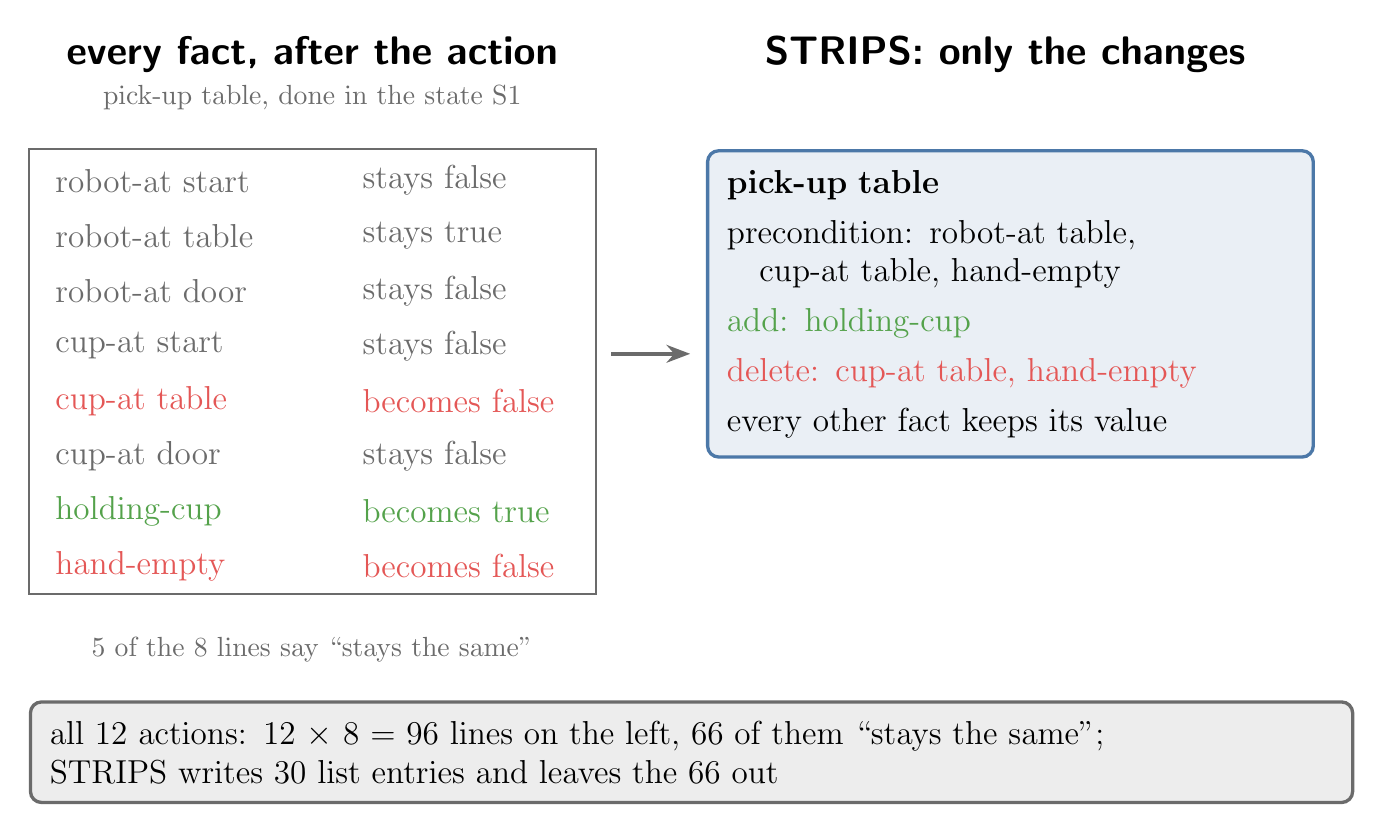
\begin{tikzpicture}[every node/.append style={font=\large}]
  \node[title] at (3.6,0.9) {every fact, after the action};
  \node[note, font=\normalsize] at (3.6,0.35) {pick-up table, done in the state S1};
  \foreach \i/\f/\w/\c in {1/robot-at start/stays false/cgrey, 2/robot-at table/stays true/cgrey,
      3/robot-at door/stays false/cgrey, 4/cup-at start/stays false/cgrey, 5/cup-at table/becomes false/cred,
      6/cup-at door/stays false/cgrey, 7/holding-cup/becomes true/cgreen, 8/hand-empty/becomes false/cred} {
    \node[anchor=west, text=\c] at (0.2,-0.7*\i) {\f};
    \node[anchor=west, text=\c] at (4.1,-0.7*\i) {\w};
  }
  \draw[cgrey, line width=0.8pt] (0,-0.3) rectangle (7.2,-5.95);
  \node[cgrey, align=center, font=\normalsize] at (3.6,-6.65) {5 of the 8 lines say ``stays the same''};

  \node[title] at (12.4,0.9) {STRIPS: only the changes};
  \node[box=cblue, anchor=north west, align=left, text width=7.2cm, font=\large] (s) at (8.6,-0.3) {
    \textbf{pick-up table}\\[4pt]
    precondition: robot-at table,\\ \quad cup-at table, hand-empty\\[4pt]
    {\color{cgreen}add: holding-cup}\\[4pt]
    {\color{cred}delete: cup-at table, hand-empty}\\[4pt]
    every other fact keeps its value};
  \draw[arrow] (7.4,-2.9) -- (8.4,-2.9);

  \node[box=cgrey, align=left, anchor=north west, text width=16.3cm, font=\large] at (0,-7.3) {
    all 12 actions: 12 $\times$ 8 = 96 lines on the left, 66 of them ``stays the same'';\\
    STRIPS writes 30 list entries and leaves the 66 out};
\end{tikzpicture}
\end{document}
